\documentclass{article}[12pt]
\usepackage{geometry}
\geometry{top=4cm,bottom=3cm,left=2cm,right=2cm}
\usepackage{guit}
\usepackage{graphicx}
\usepackage[T1]{fontenc}
\usepackage[utf8]{inputenc}
\usepackage[italian]{babel}
\usepackage{setspace}
\onehalfspacing
\title{Progetto finale\\Innovative methods to design, develop and manage complex applications}
\author{Valentina Di Mauro, Davide Carnemolla e Lorenzo Catania}


\begin{document}
	\Huge\maketitle\pagebreak
	\section[Introduzione]{Introduzione}\huge{
	Gli studenti Davide Carnemolla, Lorenzo Catania e Valentina Di Mauro presentano il seguente progetto elaborato in linea con le lezioni seminariali svoltesi durante il secondo semestre dell'anno accademico 2019-2020 e tenute da alcuni membri dell'azienda Paradigma.\\ 
	In particolare era stato richiesto di sviluppare un'applicazione client server con il framework Ionic, backend con il database non relazionale MongoDB e una tecnologia a scelta tra Angular e Node.js per il lato frontend. \\La decisione è ricaduta sull'impiego di Angular e i ruoli sono stati così divisi: Davide Carnemolla si è occupato dello sviluppo backend mentre Valentina Di Mauro e Lorenzo Catania del frontend. 
	\section{Idea del progetto}{
	Il team ha deciso di implementare un'applicazione di un albergo, denominato MewKat Palace, dove gli utenti hanno la possibilità di inserire delle recensioni e leggere e valutare quelle degli altri visitatori. \\In dettaglio le recensioni constano sia di stelle (con range da 0 a 5) che di testo.
	Coloro che leggono la recensione possono inserire un voto a favore (like) o a sfavore (dislike), indicati rispettivamente con pollice in sù e in giù.
}
	\section{Prima fase del progetto}{
	Per prima cosa il team ha ideato le Stories utilizzando la piattaforma di Trello.\\ 
		
	\begin{figure}
		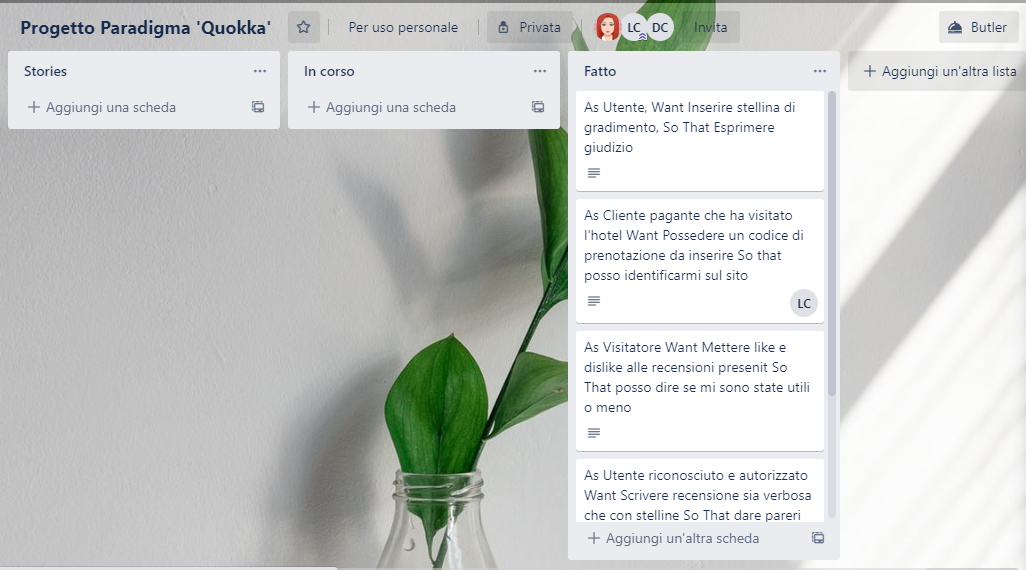
\includegraphics[width=\columnwidth]{img/storiapannello.png}
	\end{figure}
\break
	
Le storie previste, con rispettivi criteri di accettazione, sono state le seguenti:\\

	\begin{figure}
		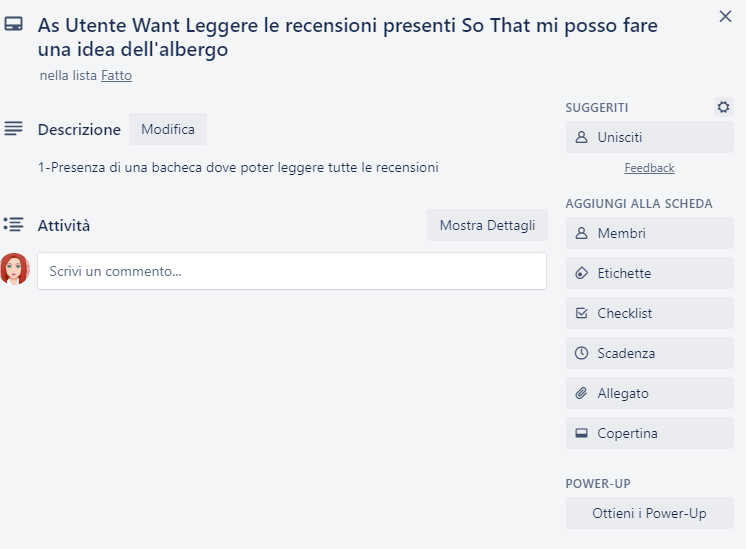
\includegraphics[width=\columnwidth]{img/storia5.png}
		\caption{As Utente, Want Leggere le recensioni presenti So That mi posso fare una idea dell'albergo}
	\end{figure}
	\begin{figure}
		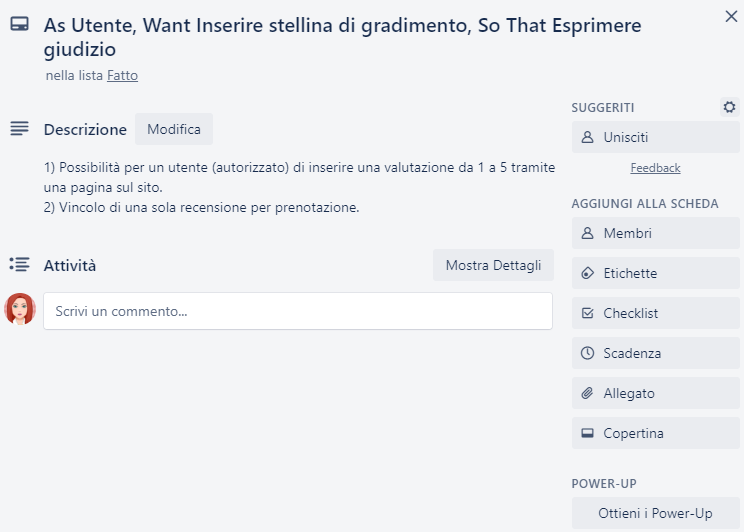
\includegraphics[width=\columnwidth]{img/storia1.png}
		\caption{As Utente, Want Inserire stellina di gradimento, So That Esprimere giudizio}
	\end{figure}
	\begin{figure}
		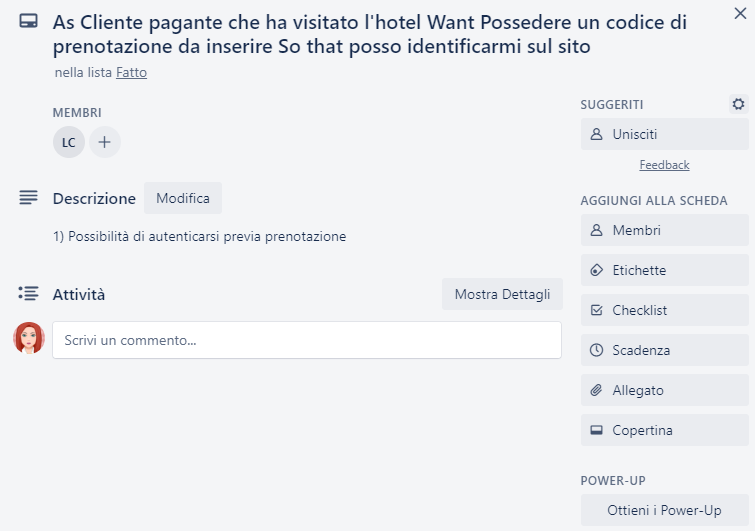
\includegraphics[width=\columnwidth]{img/storia2.png}
		\caption{As Cliente pagante che ha visitato l'hotel Want Possedere un codice di prenotazione da inserire So that posso identificarmi sul sito}
	\end{figure}
	\begin{figure}
		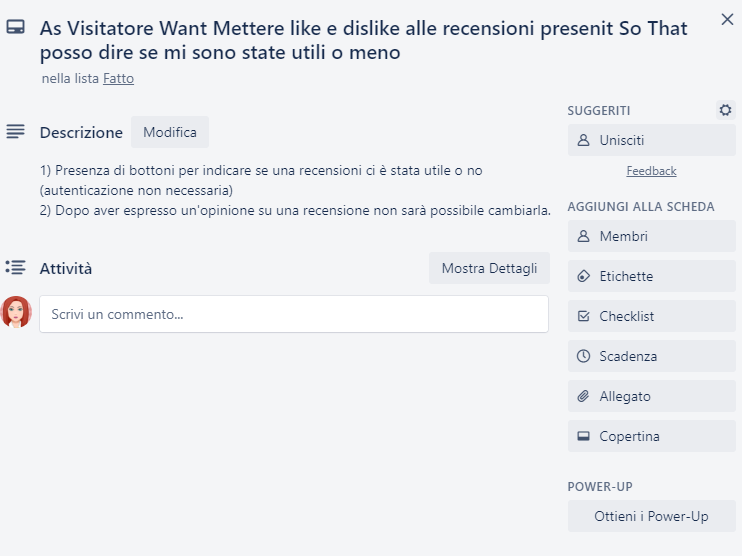
\includegraphics[width=\columnwidth]{img/storia3.png}
		\caption{As Visitatore Want Mettere like e dislike alle recensioni presenti So That posso dire se mi sono state utili o meno}
	\end{figure}
	\begin{figure}
		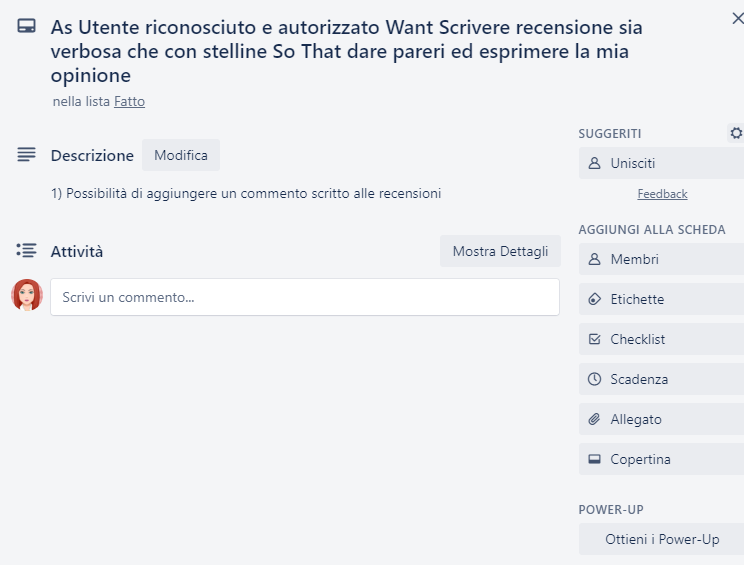
\includegraphics[width=\columnwidth]{img/storia4.png}
		\caption{As Utente riconosciuto e autorizzato Want Scrivere recensione sia verbosa che con stelline So That dare pareri ed esprimere la mia opinione}
	\end{figure}
}\break

\section{Frontend}

Gli studenti Lorenzo Catania e Valentina Di Mauro si sono riuniti per sviluppare insieme l'interfaccia utente dell'applicazione. In particolare hanno optato per utilizzare la tecnologia di Angular e rendere l'app navigabile grazie ad una struttura con Tabs.\\ La scelta è ricaduta su Angular in quanto è sembrato ad entrambi un framework molto richiesto in ambito lavorativo. \\
L'app è stata dotata di 3 Tabs: la prima rappresentante la pagina principale con presentazione dell'albergo (Home), la seconda invece risulta essere la bacheca dove poter leggere e inserire le proprie recensioni, mentre l'ultima è stata pensata come PhotoGallery.\\ Le immagini sono state prese da Pixabay così da non aver problemi di copyright. 
Come editor è stato impiegato Visual Studio Code ed è stato utilizzato GitHub per poter interagire tra i vari membri del gruppo ed assicurarsi un versioning e un backup dei sorgenti.\\ 
Come riferimento è stata consultata la documentazione ufficiale di Ionic e Angular.\\ La tab delle recensioni è stata pensata come un insieme di card dotate di bottoni. 
A seguire il frammento di codice relativo alla card sopradetta e come appare l'app con la visualizzazione in tempo reale dal Lab:\\
\begin{figure}
	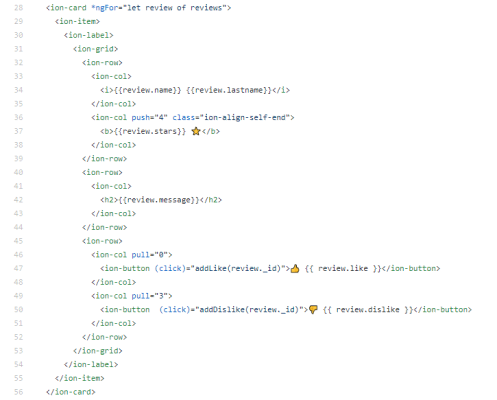
\includegraphics[height=18cm, width=\columnwidth]{img/codicecard.png}
\end{figure}

\begin{figure}
	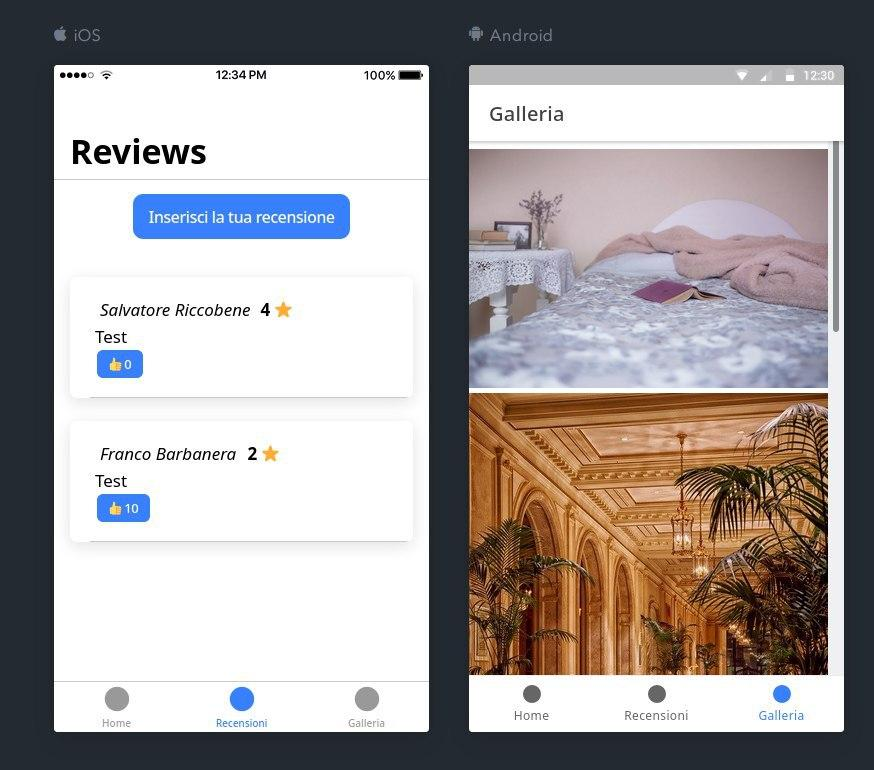
\includegraphics[width=\columnwidth]{img/screenapp.jpg}
\end{figure}\break
 
 \section{Backend}
 
 Lo studente Davide Carnemolla si è dedicato alla stesura del backend del progetto utilizzando il framework Express.js e Mongodb. Nell'applicazione vengono definiti due modelli:
 
 \begin{itemize}
 \item Review: rappresenta una recensione scritta da un utente
 \item Token: rappresenta un token generato durante la fase di prenotazione (non prevista dall'applicazione).
\end{itemize}

\noindent Per ciascuno di questi sono state definite delle route per eseguire le classiche operazioni di creazione, cancellazione, modifica e rimozione.\\
Per facilitare la fase di sviluppo e di "deployment" del progetto è stato utilizzato Docker. È possibile infatti lanciare il backend e Mongodb attraverso Docker Compose.\\
Come editor è stato utilizzato Visual Studio Code ed è stato utilizzato Github per effettuare versioning e mantenere il codice al sicuro.\\
Inoltre, per agevolare il coordinamento con gli studenti delegati allo sviluppo del frontend, è stata generata una documentazione delle REST API attraverso apidocjs.




\end{document}	